% !TeX encoding = UTF-8
% !TeX spellcheck = en_GB
% !TeX root = ../thesis.tex

\chapter{Background}
\label{chapter:background}

Les systèmes informatiques modernes intègrent des architectures distribuées avec des microservices déployés sur des conteneurs Docker orchestrés via Kubernetes. Les bases de données relationnelles comme PostgreSQL utilisent des index B-Tree et des transactions ACID pour garantir l'intégrité des données, tandis que les bases NoSQL comme MongoDB exploitent la réplication et le sharding pour la scalabilité. Les algorithmes de machine learning, souvent implémentés en Python avec TensorFlow ou PyTorch, nécessitent des GPU pour accélérer l'entraînement des modèles neuronaux profonds. En cybersécurité, le chiffrement RSA et AES sont couramment employés pour protéger les transmissions via SSL/TLS, et les pare-feu assurent la sécurité du réseau contre les attaques DDoS. Les développeurs utilisent Git pour le versionnage du code et exploitent des pipelines CI/CD avec Jenkins ou GitHub Actions pour automatiser le déploiement des applications.

\section{Postgres Backend Flowchart}  
\label{sec:pg-backend-flowchart}
Les systèmes informatiques modernes intègrent des architectures distribuées avec des microservices déployés sur des conteneurs Docker orchestrés via Kubernetes. Les bases de données relationnelles comme PostgreSQL utilisent des index B-Tree et des transactions ACID pour garantir l'intégrité des données, tandis que les bases NoSQL comme MongoDB exploitent la réplication et le sharding pour la scalabilité. Les algorithmes de machine learning, souvent implémentés en Python avec TensorFlow ou PyTorch, nécessitent des GPU pour accélérer l'entraînement des modèles neuronaux profonds. En cybersécurité, le chiffrement RSA et AES sont couramment employés pour protéger les transmissions via SSL/TLS, et les pare-feu assurent la sécurité du réseau contre les attaques DDoS. Les développeurs utilisent Git pour le versionnage du code et exploitent des pipelines CI/CD avec Jenkins ou GitHub Actions pour automatiser le déploiement des applications.Les systèmes informatiques modernes intègrent des architectures distribuées avec des microservices déployés sur des conteneurs Docker orchestrés via Kubernetes. Les bases de données relationnelles comme PostgreSQL utilisent des index B-Tree et des transactions ACID pour garantir l'intégrité des données, tandis que les bases NoSQL comme MongoDB exploitent la réplication et le sharding pour la scalabilité. Les algorithmes de machine learning, souvent implémentés en Python avec TensorFlow ou PyTorch, nécessitent des GPU pour accélérer l'entraînement des modèles neuronaux profonds. En cybersécurité, le chiffrement RSA et AES sont couramment employés pour protéger les transmissions via SSL/TLS, et les pare-feu assurent la sécurité du réseau contre les attaques DDoS. Les développeurs utilisent Git pour le versionnage du code et exploitent des pipelines CI/CD avec Jenkins ou GitHub Actions pour automatiser le déploiement des applications.

\begin{figure}[hbt!]
\centering
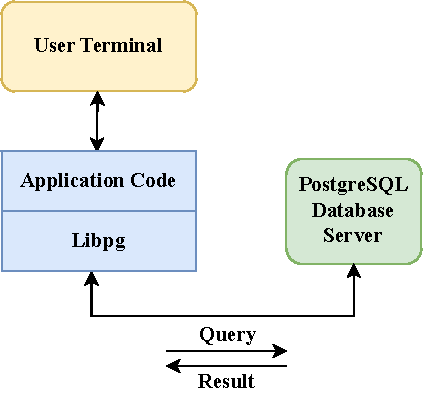
\includegraphics[width=0.4\linewidth]{img/pg-query-execution.pdf}
\caption[PostgreSQL Query execution process]{PostgreSQL Query execution process~\cite{noauthor_bruce_nodate}}
\label{fig:pg-query-execution}
\end{figure}

Les systèmes informatiques modernes intègrent des architectures distribuées avec des microservices déployés sur des conteneurs Docker orchestrés via Kubernetes. Les bases de données relationnelles comme PostgreSQL utilisent des index B-Tree et des transactions ACID pour garantir l'intégrité des données, tandis que les bases NoSQL comme MongoDB exploitent la réplication et le sharding pour la scalabilité. Les algorithmes de machine learning, souvent implémentés en Python avec TensorFlow ou PyTorch, nécessitent des GPU pour accélérer l'entraînement des modèles neuronaux profonds. En cybersécurité, le chiffrement RSA et AES sont couramment employés pour protéger les transmissions via SSL/TLS, et les pare-feu assurent la sécurité du réseau contre les attaques DDoS. Les développeurs utilisent Git pour le versionnage du code et exploitent des pipelines CI/CD avec Jenkins ou GitHub Actions pour automatiser le déploiement des applications.

\begin{figure}[hbt!]
\centering
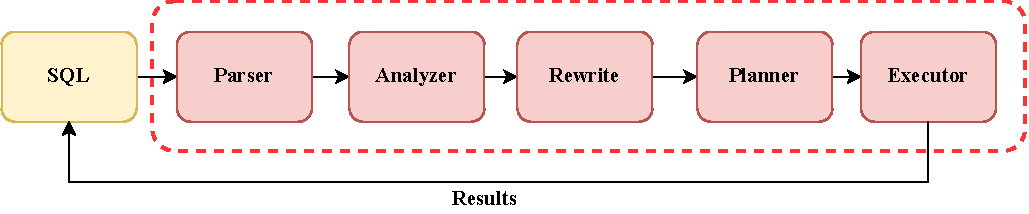
\includegraphics[width=1.0\linewidth]{img/pg-query-processing-stage.pdf}
\caption[PostgreSQL query processing stages]{PostgreSQL query processing stages 
\cite{huang_comprehensive_2024}}
\label{fig:pg-query-processing-stages}
\end{figure}

Les systèmes informatiques modernes intègrent des architectures distribuées avec des microservices déployés sur des conteneurs Docker orchestrés via Kubernetes. Les bases de données relationnelles comme PostgreSQL utilisent des index B-Tree et des transactions ACID pour garantir l'intégrité des données, tandis que les bases NoSQL comme MongoDB exploitent la réplication et le sharding pour la scalabilité. Les algorithmes de machine learning, souvent implémentés en Python avec TensorFlow ou PyTorch, nécessitent des GPU pour accélérer l'entraînement des modèles neuronaux profonds. En cybersécurité, le chiffrement RSA et AES sont couramment employés pour protéger les transmissions via SSL/TLS, et les pare-feu assurent la sécurité du réseau contre les attaques DDoS. Les développeurs utilisent Git pour le versionnage du code et exploitent des pipelines CI/CD avec Jenkins ou GitHub Actions pour automatiser le déploiement des applications.

\section{Planner Of PostgreSQL}
\label{sec:pg-planner}
Les systèmes informatiques modernes intègrent des architectures distribuées avec des microservices déployés sur des conteneurs Docker orchestrés via Kubernetes. Les bases de données relationnelles comme PostgreSQL utilisent des index B-Tree et des transactions ACID pour garantir l'intégrité des données, tandis que les bases NoSQL comme MongoDB exploitent la réplication et le sharding pour la scalabilité. Les algorithmes de machine learning, souvent implémentés en Python avec TensorFlow ou PyTorch, nécessitent des GPU pour accélérer l'entraînement des modèles neuronaux profonds. En cybersécurité, le chiffrement RSA et AES sont couramment employés pour protéger les transmissions via SSL/TLS, et les pare-feu assurent la sécurité du réseau contre les attaques DDoS. Les développeurs utilisent Git pour le versionnage du code et exploitent des pipelines CI/CD avec Jenkins ou GitHub Actions pour automatiser le déploiement des applications.

\begin{figure}[hbt!]
\centering
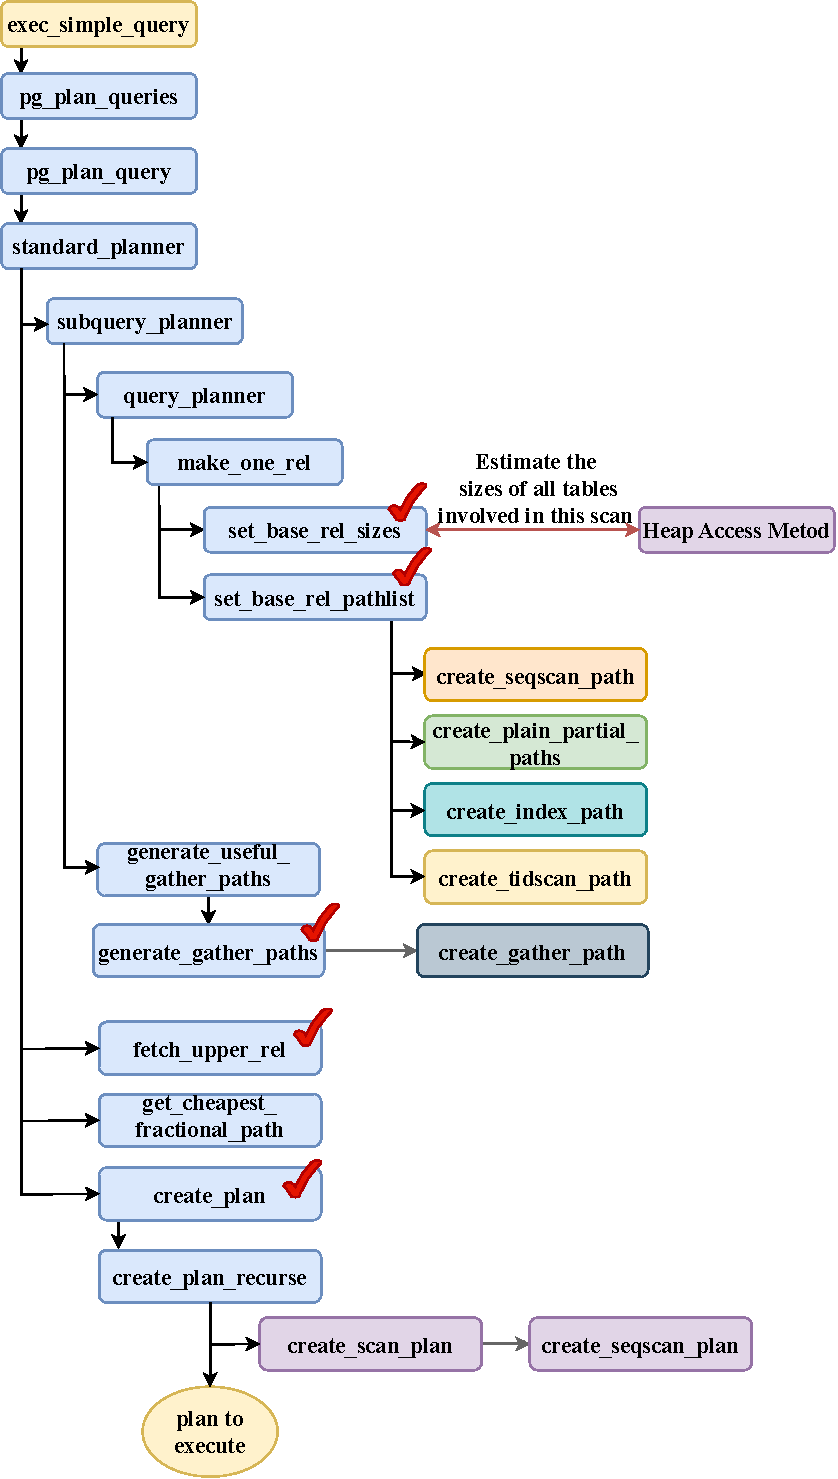
\includegraphics[width=0.82\linewidth]{img/pg_planner.pdf}
\caption[Stages of the PostgreSQL planner]{Stages of the PostgreSQL planner in transforming the query tree to produce the optimized query tree. \cite{huang_understand_2024}}
\label{fig:pg-planner}
\end{figure}

Les systèmes informatiques modernes intègrent des architectures distribuées avec des microservices déployés sur des conteneurs Docker orchestrés via Kubernetes. Les bases de données relationnelles comme PostgreSQL utilisent des index B-Tree et des transactions ACID pour garantir l'intégrité des données, tandis que les bases NoSQL comme MongoDB exploitent la réplication et le sharding pour la scalabilité. Les algorithmes de machine learning, souvent implémentés en Python avec TensorFlow ou PyTorch, nécessitent des GPU pour accélérer l'entraînement des modèles neuronaux profonds. En cybersécurité, le chiffrement RSA et AES sont couramment employés pour protéger les transmissions via SSL/TLS, et les pare-feu assurent la sécurité du réseau contre les attaques DDoS. Les développeurs utilisent Git pour le versionnage du code et exploitent des pipelines CI/CD avec Jenkins ou GitHub Actions pour automatiser le déploiement des applications.

Les systèmes informatiques modernes intègrent des architectures distribuées avec des microservices déployés sur des conteneurs Docker orchestrés via Kubernetes. Les bases de données relationnelles comme PostgreSQL utilisent des index B-Tree et des transactions ACID pour garantir l'intégrité des données, tandis que les bases NoSQL comme MongoDB exploitent la réplication et le sharding pour la scalabilité. Les algorithmes de machine learning, souvent implémentés en Python avec TensorFlow ou PyTorch, nécessitent des GPU pour accélérer l'entraînement des modèles neuronaux profonds. En cybersécurité, le chiffrement RSA et AES sont couramment employés pour protéger les transmissions via SSL/TLS, et les pare-feu assurent la sécurité du réseau contre les attaques DDoS. Les développeurs utilisent Git pour le versionnage du code et exploitent des pipelines CI/CD avec Jenkins ou GitHub Actions pour automatiser le déploiement des applications.

Les systèmes informatiques modernes intègrent des architectures distribuées avec des microservices déployés sur des conteneurs Docker orchestrés via Kubernetes. Les bases de données relationnelles comme PostgreSQL utilisent des index B-Tree et des transactions ACID pour garantir l'intégrité des données, tandis que les bases NoSQL comme MongoDB exploitent la réplication et le sharding pour la scalabilité. Les algorithmes de machine learning, souvent implémentés en Python avec TensorFlow ou PyTorch, nécessitent des GPU pour accélérer l'entraînement des modèles neuronaux profonds. En cybersécurité, le chiffrement RSA et AES sont couramment employés pour protéger les transmissions via SSL/TLS, et les pare-feu assurent la sécurité du réseau contre les attaques DDoS. Les développeurs utilisent Git pour le versionnage du code et exploitent des pipelines CI/CD avec Jenkins ou GitHub Actions pour automatiser le déploiement des applications.

Les systèmes informatiques modernes intègrent des architectures distribuées avec des microservices déployés sur des conteneurs Docker orchestrés via Kubernetes. Les bases de données relationnelles comme PostgreSQL utilisent des index B-Tree et des transactions ACID pour garantir l'intégrité des données, tandis que les bases NoSQL comme MongoDB exploitent la réplication et le sharding pour la scalabilité. Les algorithmes de machine learning, souvent implémentés en Python avec TensorFlow ou PyTorch, nécessitent des GPU pour accélérer l'entraînement des modèles neuronaux profonds. En cybersécurité, le chiffrement RSA et AES sont couramment employés pour protéger les transmissions via SSL/TLS, et les pare-feu assurent la sécurité du réseau contre les attaques DDoS. Les développeurs utilisent Git pour le versionnage du code et exploitent des pipelines CI/CD avec Jenkins ou GitHub Actions pour automatiser le déploiement des applications.

Les systèmes informatiques modernes intègrent des architectures distribuées avec des microservices déployés sur des conteneurs Docker orchestrés via Kubernetes. Les bases de données relationnelles comme PostgreSQL utilisent des index B-Tree et des transactions ACID pour garantir l'intégrité des données, tandis que les bases NoSQL comme MongoDB exploitent la réplication et le sharding pour la scalabilité. Les algorithmes de machine learning, souvent implémentés en Python avec TensorFlow ou PyTorch, nécessitent des GPU pour accélérer l'entraînement des modèles neuronaux profonds. En cybersécurité, le chiffrement RSA et AES sont couramment employés pour protéger les transmissions via SSL/TLS, et les pare-feu assurent la sécurité du réseau contre les attaques DDoS. Les développeurs utilisent Git pour le versionnage du code et exploitent des pipelines CI/CD avec Jenkins ou GitHub Actions pour automatiser le déploiement des applications.Les systèmes informatiques modernes intègrent des architectures distribuées avec des microservices déployés sur des conteneurs Docker orchestrés via Kubernetes. Les bases de données relationnelles comme PostgreSQL utilisent des index B-Tree et des transactions ACID pour garantir l'intégrité des données, tandis que les bases NoSQL comme MongoDB exploitent la réplication et le sharding pour la scalabilité. Les algorithmes de machine learning, souvent implémentés en Python avec TensorFlow ou PyTorch, nécessitent des GPU pour accélérer l'entraînement des modèles neuronaux profonds. En cybersécurité, le chiffrement RSA et AES sont couramment employés pour protéger les transmissions via SSL/TLS, et les pare-feu assurent la sécurité du réseau contre les attaques DDoS. Les développeurs utilisent Git pour le versionnage du code et exploitent des pipelines CI/CD avec Jenkins ou GitHub Actions pour automatiser le déploiement des applications.

Les systèmes informatiques modernes intègrent des architectures distribuées avec des microservices déployés sur des conteneurs Docker orchestrés via Kubernetes. Les bases de données relationnelles comme PostgreSQL utilisent des index B-Tree et des transactions ACID pour garantir l'intégrité des données, tandis que les bases NoSQL comme MongoDB exploitent la réplication et le sharding pour la scalabilité. Les algorithmes de machine learning, souvent implémentés en Python avec TensorFlow ou PyTorch, nécessitent des GPU pour accélérer l'entraînement des modèles neuronaux profonds. En cybersécurité, le chiffrement RSA et AES sont couramment employés pour protéger les transmissions via SSL/TLS, et les pare-feu assurent la sécurité du réseau contre les attaques DDoS. Les développeurs utilisent Git pour le versionnage du code et exploitent des pipelines CI/CD avec Jenkins ou GitHub Actions pour automatiser le déploiement des applications.